%%% template.annotated.tex
%%%
%%% This LaTeX source document can be used as the basis for your technical
%%% paper or abstract. Unlike ``template.tex,'' this version of the source
%%% document contains documentation of each of the commands and definitions
%%% that should be used in the preparation of your formatted document.
%%% 
%%% The parameter given to the ``acmsiggraph'' LaTeX class in the 
%%% ``\documentclass'' command controls several features of the formatted 
%%% output: the presence or absence of hyperlinked icons just prior to the 
%%% first section of the paper, the amount of space left clear for the ACM
%%% copyright notice, the presence or absence of line numbers and submission
%%% ID, and the presence or absence of an appropriate ``preprint'' notice.
%%% 
%%% If you are preparing a paper for presentation in the Technical Papers
%%% program at one of our two annual flagship conferences, held in North 
%%% America (SIGGRAPH) or Asia (SIGGRAPH Asia), you should use ``tog''
%%% as the parameter.
%%%
%%% If you are preparing a paper for presentation at one of our sponsored
%%% events, including SIGGRAPH and SIGGRAPH Asia, but not in those events' 
%%% Technical Papers program, or a one- to four-page abstract, you should 
%%% use ``conference'' as the parameter.
%%% (Technical Briefs and Game Papers presented at our annual flagship 
%%% events fall into this category, as do papers accepted to other SIGGRAPH-
%%% sponsored events, such as I3D or ETRA or VRCAI, as do the one-page 
%%% abstracts which serve as the primary documentation for many of our 
%%% annual conference programs, including Posters, Talks, and Emerging 
%%% Technologies.)
%%%
%%% If you are preparing a version of your content for review, you should
%%% use ``review'' as the parameter. Line numbers will be added to your 
%%% paper, and the submission ID value will be printed across the top of 
%%% each page of your paper. (Use the submission ID as the parameter to the
%%% ``TOGonlineID'' command, below.)
%%%
%%% If you are preparing a preprint of your content, you should use
%%% ``preprint'' as the parameter. This is primarily for annual conference
%%% papers; a header reading ``To appear in ACM TOG X(Y)'' will appear on
%%% each page of the formatted output (where X is the volume and Y is the 
%%% number of the issue in which it will be published).

\documentclass[tog]{acmsiggraph}

\usepackage{siunitx}

%%% Definitions and commands that begin with ``\TOG'' are meant to be used
%%% in the preparation of papers to be presented in the Technical Papers
%%% program at one of our annual flagship events - SIGGRAPH and SIGGRAPH 
%%% Asia. You can safely ignore these definitions and commands if your 
%%% content is to be presented in some other venue.

%%% ``\TOGonlineid'' should be filled with the online ID value you received
%%% when you submitted your technical paper. It will be printed out if you 
%%% prepare a ``review'' version of your paper.

\TOGonlineid{45678}

%%% Should your technical paper be accepted, you will be given three pieces
%%% of information: the volume and number of the issue of the ACM Transactions
%%% on Graphics journal in which your paper will be published, and the 
%%% ``article DOI'' value, which is unique to your paper and provides the 
%%% link to your paper's page in the ACM Digital Library. Fill in the 
%%% ``\TOGvolume,'' ``\TOGnumber,'' and ``\TOGarticleDOI'' definitions with
%%% the three pieces of information you receive.

\TOGvolume{0}
\TOGnumber{0}
\TOGarticleDOI{1111111.2222222}

%%% By default, your technical paper will contain hyperlinked icons which 
%%% point to your paper's article page in the ACM Digital Library, and to 
%%% the paper itself in the ACM Digital Library. You may wish to add one 
%%% or more links to your own resources. If any of the following four 
%%% definitions have URLs in them, an appropriate hyperlinked icon will be
%%% added to the list. 

\TOGprojectURL{}
\TOGvideoURL{}
\TOGdataURL{}
\TOGcodeURL{}

%%% Define the title of your paper here. Use capital letters as appropriate.
%%% Setting the entire title in upper-case letters is not correct, nor is 
%%% capitalizing only the first letter of the title.

\title{Simulating Magnets}

%%% Define the author list in the ``\author'' command. The ``\thanks'' 
%%% field can be used to define an e-mail address for the author.
%%% The ``\pdfauthor'' field should contain a comma-separated list of the
%%% authors of the paper, and is used, along with the title and keyword
%%% data, for PDF metadata. (To see this metadata, open the PDF in Adobe 
%%% Reader and select ``File > Properties > Description.''

\author{Richard DeVries\thanks{e-mail:rdevries@student.cs.uwaterloo.ca}\\University of Waterloo}
\pdfauthor{Richard DeVries}

%%% User-defined keywords.

\keywords{magnet, magnetic induction, rigid body dynamics}

%%% End of the document preamble, start of the document.

\begin{document}

%%% A ``teaser'' image appears below the title and affiliation and above
%%% the two-column body of the paper. This is optional, but if you wish
%%% to include such an image, the commented-out code, below, can be used
%%% as an example. Please note that the inclusion of a ``teaser'' image
%%% may move the copyright space to the bottom of the right-hand column
%%% on the first page of your formatted output. This is acceptable.

 \teaser{
   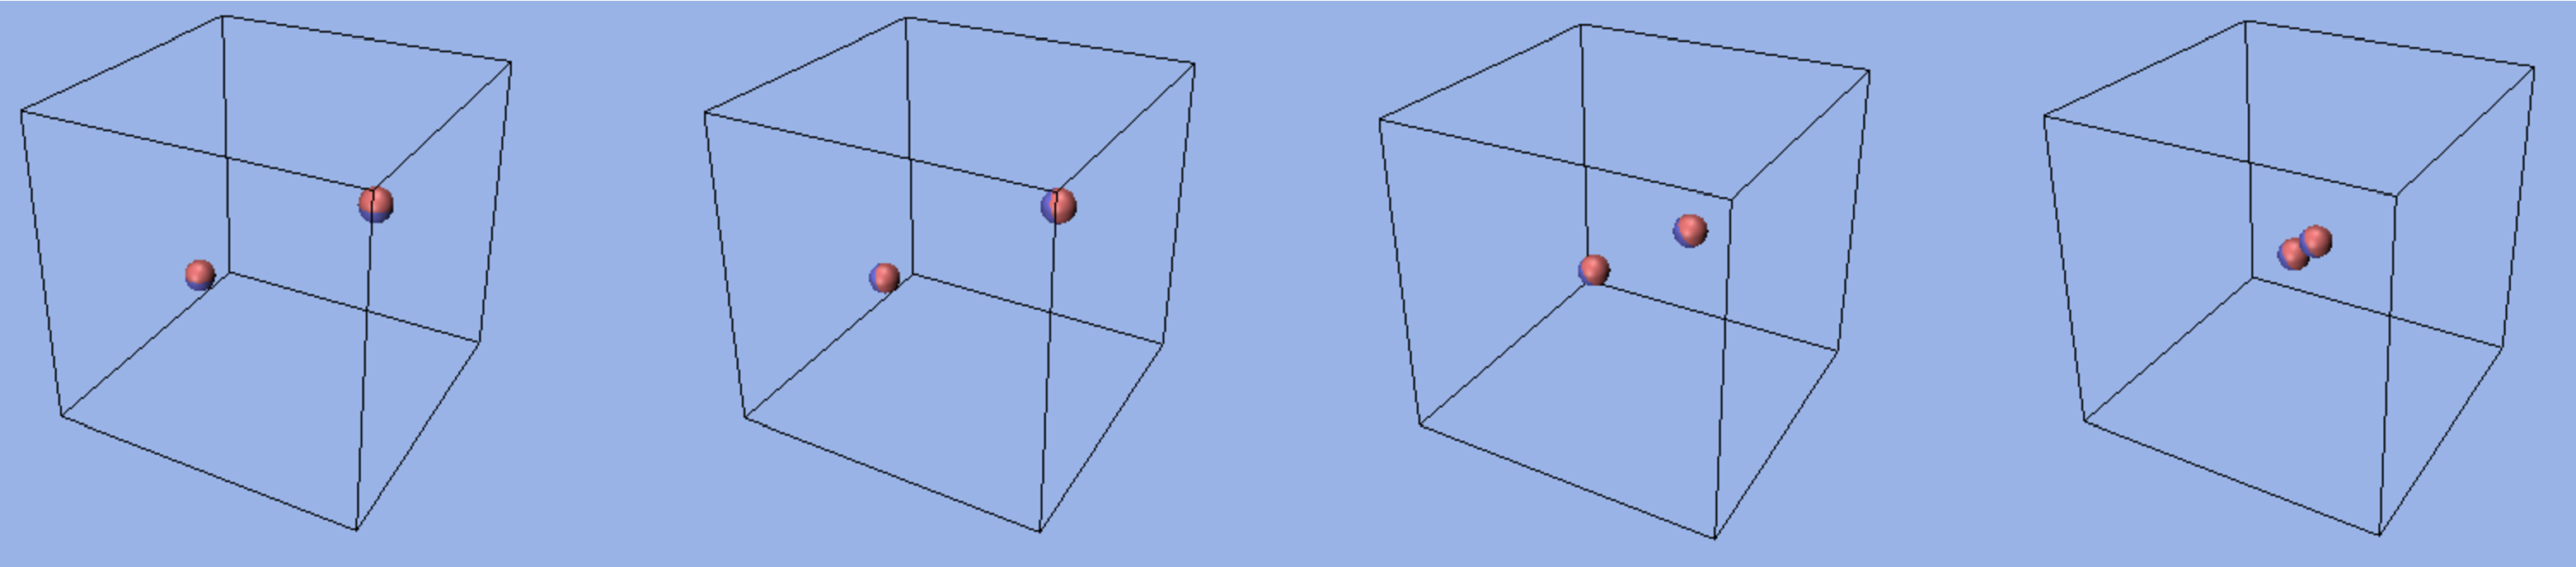
\includegraphics[height=1.5in]{images/MagnetImage1}
   \caption{Two magnets rotate to align their opposing poles and move towards each other}
 }

%%% The ``\maketitle'' command uses the author and title information 
%%% defined above, and prepares the formatted title.

\maketitle

%%% The ``abstract'' environment should contain the abstract for your
%%% content -- one to several paragraphs which describe the work.

\begin{abstract}

This report describes the physics-based animation concepts required to transform a simple particle simulator into a somewhat less simple magnet simulator. In particular, there are four concepts required to perform this transformation. First, since magnets attract each other, they will inevitably come into contact. This requires collision detection and handling. Second, magnets rotate and move about during the simulation. This requires implementing the rigid body equations of motion. Third, magnetic forces and torques need to be calculated so that the motion of the magnets can be determined. To do this, the magnetic induction caused by the magnets at arbitrary points must be calculated. The magnetic induction can also be used to draw magnetic field lines. Finally, the magnetic forces and torques can be calculated and applied to the magnets.

%Citations can be done this way~\cite{Jobs95} or this more concise 
%way~\shortcite{Jobs95}, depending upon the application.

\end{abstract}

%%% The ``CRCatlist'' environment defines one or more ACM ``Computing Review''
%%% (or ``CR'') categories, used for indexing your work. For more information
%%% on CR categories, please see http://www.acm.org/class/1998.

\begin{CRcatlist}
  \CRcat{I.3.5}{Computer Graphics}{Computational Geometry and Object Modelling}{Physically Based Modelling}.
\end{CRcatlist}

%%% The ``\keywordlist'' prints out the user-defined keywords.

\keywordlist

%%% If you are preparing a paper to be presented in the Technical Papers
%%% program at one of our annual flagship events (and, therefore, using 
%%% the ``tog'' parameter to the ``\documentclass'' command), the 
%%% ``\TOGlinkslist'' command prints out the list of hyperlinked icons.
%%% If you are using any other parameter to the ``\documentclass'' command
%%% this command does absolutely nothing.

%\TOGlinkslist

%%% The ``\copyrightspace'' command will leave clear an amount of space
%%% at the bottom of the left-hand column on the first page of your paper,
%%% according to the parameter used in the ``\documentclass'' command.

\copyrightspace

%%% The first section of your paper. 

\section{Introduction}

Magnets and magnetic objects are frequently encountered in real life. Fridge magnets are used to attach shopping lists to the fridge, magnets are used in various electronics like computer hard drives, and there are children's toys that make use of metal balls and plastic rods with magnets on the ends. Despite how common magnets are, however, there are not many papers in the computer graphics community that explore magnetism. This report aims to give an overview of the basic concepts required to create a magnet simulator.

As this report presents merely the basics of a magnet simulator, not everything about simulating magnets and magnetism will be covered. Objects with permanent magnetization (that is, objects that induce a magnetic field on their own) are covered in this report, whereas objects with induced magnetization (that is, objects that become magnetic when exposed to a magnetic field) are not. In terms of the children's toy with the metal balls and plastic rods with magnets on the ends, the magnets in the plastic rods have permanent magnetization, whereas the metal balls have induced magnetization. This can be seen by the interaction between two of the metal balls. By themselves, two of the metal balls will not attract each other; however, when one of the metal balls is attached to the end of one of the plastic rods, the metal balls will stick to each other because of the induced magnetization in the balls. If the reader is interested in learning about objects with induced magnetization, they are encouraged to read ~\cite{Thomaszewski:2008:MIM}.

The remainder of this report proceeds as follows. Section 2 briefly describes the work that this report is based on. Section 3 will describe the rigid body dynamics concepts used in this project. Section 4 will describe the magnetism concepts used in this project. Section 5 will present and discuss some animations produced by this project. Finally, section 6 will discuss some shortcomings of this project and some future work that would improve it.

\section{Previous Work}

Rigid body simulation is a much-explored area of physics-based animation. However, for this project, only some basic parts of rigid body animation are required, so this project uses the 2001 online SIGGRAPH course notes ~\cite{pixarnotes} for the required background on rigid body animation. These course notes give an excellent introduction to many aspects of physically-based modelling, including differential equations, particle dynamics, rigid body dynamics, collision detection and handling, and a few others. The sections on rigid body dynamics and collision detection and handling are the most important sections of the course notes for this project.

As mentioned above, there has not been a lot of research into simulating magnets in the computer graphics community. One paper that does explore magnetism is ~\cite{Thomaszewski:2008:MIM}. That paper covers the basics of magnets, including calculating magnetic induction and the forces and torques applied by the magnetic fields. This is the part of that paper that is implemented in this project. That paper also covers induced magnetism, which is not implemented in this project, as mentioned above. One further interesting topic explored by that paper is superconductors and their interaction with magnets.

\section{Rigid Body Dynamics}

We now go into detail about the rigid body dynamics concepts required for this project. As this project is focused on the basics, the description of these concepts will be primarily focused on one of the most basic shapes, the sphere. Some high-level explanation of how to extend these ideas to more general shapes will also be given.

\subsection{Collision Detection and Handling}

The first concept from rigid body dynamics that is explained is collision detection and handling. This is important for a magnet simulator because, in many circumstances, magnets will come into contact at some point in the simulation. If the collisions are not handled, the simulation will be highly physically inaccurate.

Before the positions and velocities of objects can be adjusted to account for collisions, the collisions must be detected. For spheres, detecting collisions is quite simple: if the distance between the centres of two spheres is less than the sum of their radii, then the spheres are intersecting, so they have collided.

For other shapes, collision detection is more complicated because other shapes are not as uniform as spheres. For general convex polyhedra, one method of testing for intersections is separating planes. As explained in ~\cite{pixarnotes}, if two convex polyhedra are non-intersecting, ``then a separating plane exists with the following property: either the plane contains a face of one of the polyhedra, or the plane contains an edge from one of the polyhedra and is parallel to an edge of the other polyhedra.'' Although finding these separating planes can take quite a bit of time, they can frequently be reused, so they do not need to be found at every time step. For more information on general collision detection, see Section 7 of the Rigid Body Dynamics chapter of ~\cite{pixarnotes}.

One method of handling the collisions is using penalty forces. This method allows objects to inter-penetrate, but when they do, a force is applied to the two objects to push them apart. This force is proportional to the distance the objects have inter-penetrated, so that the more the objects overlap, the stronger the force is that pushes them apart. That is, the force applied on object A for overlapping object B is:
\begin{equation}
 F = kd\hat{n}
\end{equation}
where $k$ is a constant that can be adjusted to produce softer or harder collisions, $d$ is the distance that object A has penetrated into object B, and $\hat{n}$ is the unit vector normal to the surface of B at the point of the collision. For two colliding spheres, $d$ is the sum of the radii of the spheres minus the distance between the centres of the two spheres, and $\hat{n}$ is the unit vector pointing from the centre of one sphere to the centre of the other. The direction of $\hat{n}$ is chosen based on which sphere's penalty force is being calculated.

\subsection{Rigid Body Equations of Motion}

The second concept from rigid body dynamics that is crucial for a magnet simulator is the set of equations describing rigid body motion. These equations allow the simulated magnets to rotate so that opposing poles can align and to move towards and away from each other as the magnetic forces dictate.

It is useful to first look at what information is required to advance a rigid body in a simulator. As rigid bodies do not change their shape as the simulation progresses, their motion can be considered a combination of translations of and rotations about the centre of mass of the object. To update these throughout a simulation, it is necessary to store some information about the current state of the translations and rotations, as well as some information about how the translations and rotations are changing. This can be done by storing the following four pieces of information: the location of the centre of mass $x(t)$ of the rigid body, a rotation matrix $R(t)$ defining the orientation of the rigid body (quaternions are generally preferred for this, but for simplicity, we stick with a rotation matrix), the linear momentum $P(t)$ of the rigid body, and the angular momentum $L(t)$ of the rigid body.

To update these values from one time step to the next, the derivatives of these values are required. Though it may possibly seem strange that linear and angular momentums are stored rather than linear and angular velocities, the required derivatives are quite simple to calculate this way. By the definition of linear momentum:
\begin{equation}
 v(t) = \frac{P(t)}{m}
\end{equation}
where $m$ is the mass of the rigid body. This gives the derivative of $x(t)$. Additionally, the derivative of $P(t)$ is simply $F(t)$, the sum of the forces applied to the object, and the derivative of $L(t)$ is simply $\tau(t)$, the sum of the torques applied to the object.

Finding the derivative of the rotation matrix is a bit more complicated. First, the inertia tensor $I(t)$ is required. As described in ~\cite{pixarnotes}, this is ``the scaling factor between angular momentum [...] and angular velocity''. This inertia tensor is dependent on the rotation of the object, though it can be computed easily as
\begin{equation}
 I(t) = R(t)I_{body}R(t)^{T}
\end{equation}
where $R(t)$ is the rotation matrix defining the orientation of the object and $I_{body}$ is the inertia tensor of the unrotated object. For a solid sphere,
\begin{equation}
 I_{body} =
   \begin{bmatrix}
   	\frac{2}{5}mr^2 & 0 & 0\\
   	0 & \frac{2}{5}mr^2 & 0\\
   	0 & 0 & \frac{2}{5}mr^2\\
   \end{bmatrix}
\end{equation}
where $m$ is the mass and $r$ is the radius of the sphere.

Now that the inertia tensor $I(t)$ has been found, the angular velocity $\omega(t)$ can be found:
\begin{equation}
\omega(t) = I(t)^{-1}L(t)
\end{equation}
Since finding matrix inverses can be costly, this can be implemented more efficiently by noting that, for rotation matrices,
\begin{equation}
R(t)^{T} = R(t)^{-1}
\end{equation}
which gives:
\begin{equation}
I(t)^{-1} = (R(t)I_{body}R(t)^{T})^{-1} = R(t)I_{body}^{-1}R(t)^{T}
\end{equation}
Since $I_{body}$ is constant for a rigid body, so is $I_{body}^{-1}$, so this matrix inverse only needs to be calculated once.

Finally, the derivative of the rotation matrix can be found, which is $\omega(t)^{\star}R(t)$.

Having found the derivatives of the four values stored for each rigid body, any time integration scheme can be used to advance the rigid bodies through the simulation.

For additional detail on how these values are calculated, as well as a discussion on using quaternions rather than rotation matrices, see sections 2, 3, and 4 of the Rigid Body Dynamics chapter of ~\cite{pixarnotes}.

\section{Magnet Simulation}

The basic concepts of magnetism required to simulate magnets are now described.

\subsection{Calculating Magnetic Induction}

In order to simulate magnets, the forces and torques applied by the magnets need to be calculated. However, computing the magnetic forces and torques relies on finding the magnetic induction, so this is covered first.

We first consider the case of a small magnetic dipole. Let $r_O$ be the location of the dipole, and let the vector $m$ be the magnetic moment of the dipole. The length of $m$ defines the strength of the magnetic dipole, and the direction of $m$ is the direction in which the north pole of the dipole points. Then the magnetic induction $B(r)$ caused by this magnetic dipole at any point $r$ is:
\begin{equation}
B(r) = \frac{\mu_0}{4\pi}\left[\frac{3n(n\cdot m) - m}{\left|r - r_O\right|^3}\right]
\end{equation}
where $n$ is a unit vector pointing in the same direction as $(r - r_O)$. $\mu_0$ is the magnetic constant \SI[per-mode=fraction]{4\pi e-7}{\volt \second \per \ampere \per \metre}.

This equation can be used to approximate the magnetic induction caused by magnets with volume. Large magnets can be divided up into many smaller components, with each component's magnetic properties being treated as a dipole at its centre.

Given a set of magnets, the total magnetic induction at a point can be found by simply summing the magnetic inductions caused by each component of each magnet. Since the total magnetic induction can be found at any point in the scene, and since this magnetic induction is a vector, any iterative method can be used to draw a series of line segments approximating the magnetic induction lines. This produces the familiar loops often seen in diagrams of magnetic fields. In the examples below, starting points were chosen on the magnets, and an explicit forward Euler iterative scheme was used to determine the drawn magnetic field lines.

\subsection{Calculating Magnetic Forces and Torques}

As explained in ~\cite{Thomaszewski:2008:MIM}, the force $F$ and torque $T$ applied by a magnetic induction $B$ on a dipole with magnetic moment $m$ are approximated by:
\begin{equation}
F = \nabla(m \cdot B)
\end{equation}
\begin{equation}
T = m \times B
\end{equation}

These two equations can be combined with the above calculation of $B(r)$ by summing (8) over all components of all magnets that are not the magnet that the forces and torques are being calculated for. This gives the following equations for calculating the magnetic forces and torques applied to a component $k$ of a magnet:
\begin{equation}
\begin{split}
F_k = \frac{\mu_0}{4\pi}\sum_{i=1}^N \frac{1}{\left|r_k - r_i\right|^4}\left[-15n_{ik}\bigl((m_k \cdot n_{ik})(m_i \cdot n_{ik})\bigr) \right. \\
\left. + 3n_{ik}(m_k \cdot m_i) + 3\bigl(m_k(m_i \cdot n_{ik}) + m_i(m_k \cdot n_{ik})\bigr)\right]
\end{split}
\end{equation}
\begin{equation}
T_k = \frac{\mu_0}{4\pi}\sum_{i=1}^N \left[ \frac{3(m_k \times n_{ik})(m_i \cdot n_{ik}) - m_k \times m_i}{\left| r_k - r_i \right|^3} \right]
\end{equation}
Note that subscripts of $k$ indicate values corresponding to the magnet component $k$. Also note that the summation is over the components of the magnets that do not contain the magnet component $k$. As in the previous equations, $r_j$ is the location of the magnet component $j$, and $m_j$ is the magnetic moment of the magnet component $j$. $n_{ik}$ is the unit vector pointing from the location of the magnet component $i$ to the location of the magnet component $k$.

One interesting thing to note about these equations is the exponent on the $\frac{1}{\left|r_k - r_i\right|}$ factor. For the force equation, the exponent is $4$, while in the torque equation, the exponent is $3$. Thus, if two magnets are far apart, the torque will dominate the force. This causes the magnets to rotate, aligning opposite poles, more than move towards each other. This can be seen in the third example animation discussed in the next section.

For further information about calculating magnetic induction, forces, and torques, an interested reader is encouraged to see ~\cite{Thomaszewski:2008:MIM}.

\section{Results}

The results shown in the included video are now discussed. In all of the animations, the wireframe cube has a side length of 1 metre. The spheres have a radius of 5 centimetres, a mass of 1 kilogram, and a magnetic moment of 300 joules per tesla. Each component of the horseshoe magnet in the final animation also has a magnetic moment of 300 joules per tesla. For each animation, around 100 time steps were used for each second of animation, and each second of animation corresponds to approximately 0.1 seconds in the simulation. That is, the animations are shown at one-tenth speed.

The first animation is of three single-component, spherical magnets in a line. These magnets are aligned so that they are all attracted towards each other. Since the magnets are evenly spaced out, the centre magnet stays stationary, as expected. When the magnets come into contact, the penalty forces push them apart again. After the second contact, the magnets bounce farther apart than they did after the first contact. The reason for this oddity is discussed in the next section.

The second animation is similar to the first animation, except the spheres are not evenly spaced, and they are aligned to repulse each other. Note that for this animation, the magnetic induction lines tend to loop back to the opposite pole of the same magnet, rather than go to the opposing pole of a different magnet, as they do in the first animation. This is how the magnetic field lines are expected to look for repulsing magnets.

\begin{figure}[ht]
  \centering
  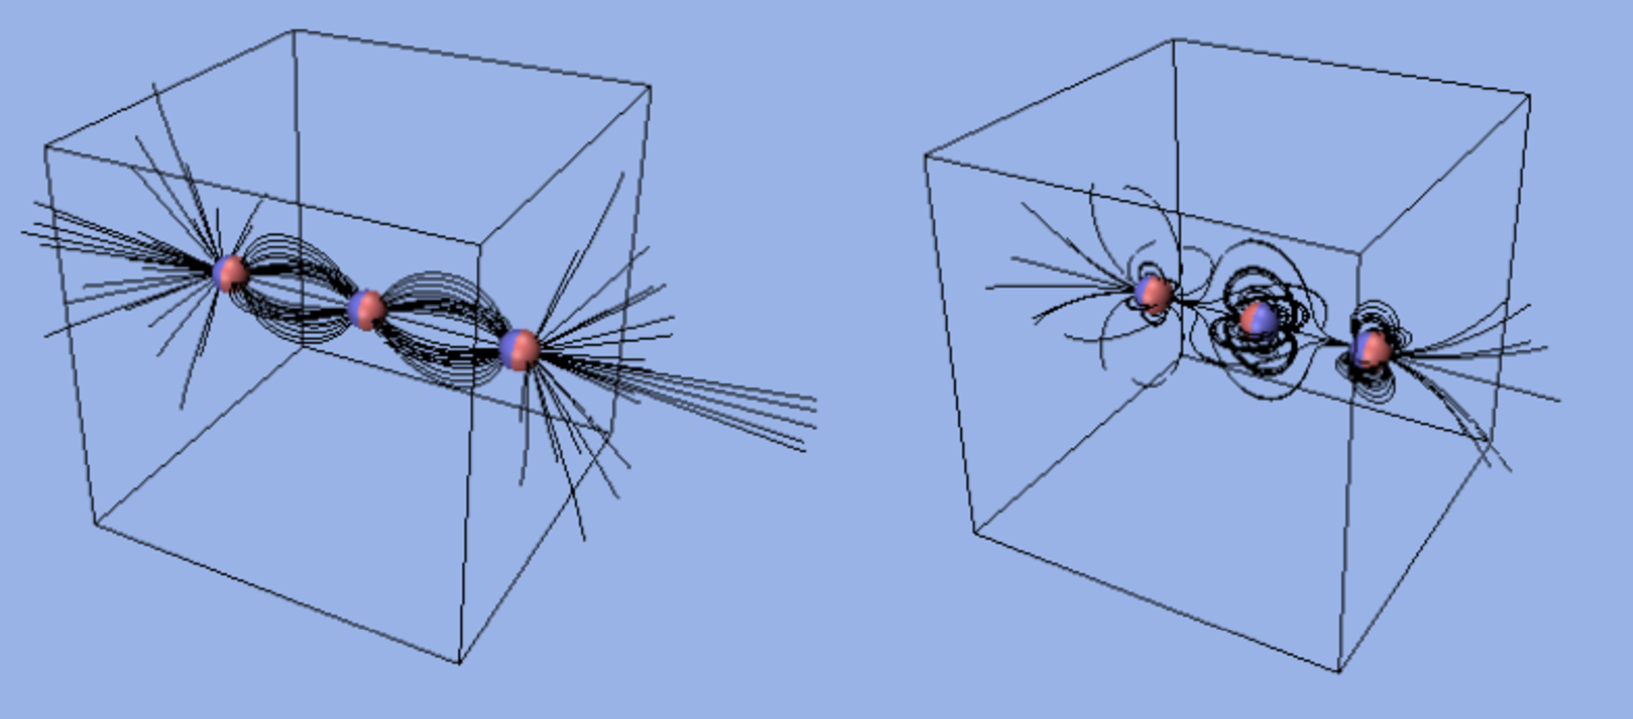
\includegraphics[width=3.0in]{images/MagnetImage2}
  \caption{The magnetic field lines for attracting (left) and repulsing (right) magnets}
\end{figure}

The third animation demonstrates how, when two magnets are far apart, the interaction between them is dominated by the torques. In this animation, the magnets turn so that their opposing poles are facing each other much faster than the magnets move towards each other. One might notice that when the two magnets collide, they bounce back much less than the magnets do in the first animation. Again, the reason for this is discussed in the following section.

The final animation shows a stationary, multi-component horseshoe magnet and a single-component spherical magnet. The magnet is placed an equal distance from the two ends of the horseshoe magnet. This results in the horizontal magnetic forces on the sphere cancelling out, causing the sphere to oscillate up and down. Because there is no force damping the spherical magnet's motion, it oscillates indefinitely.

\begin{figure}[ht]
  \centering
  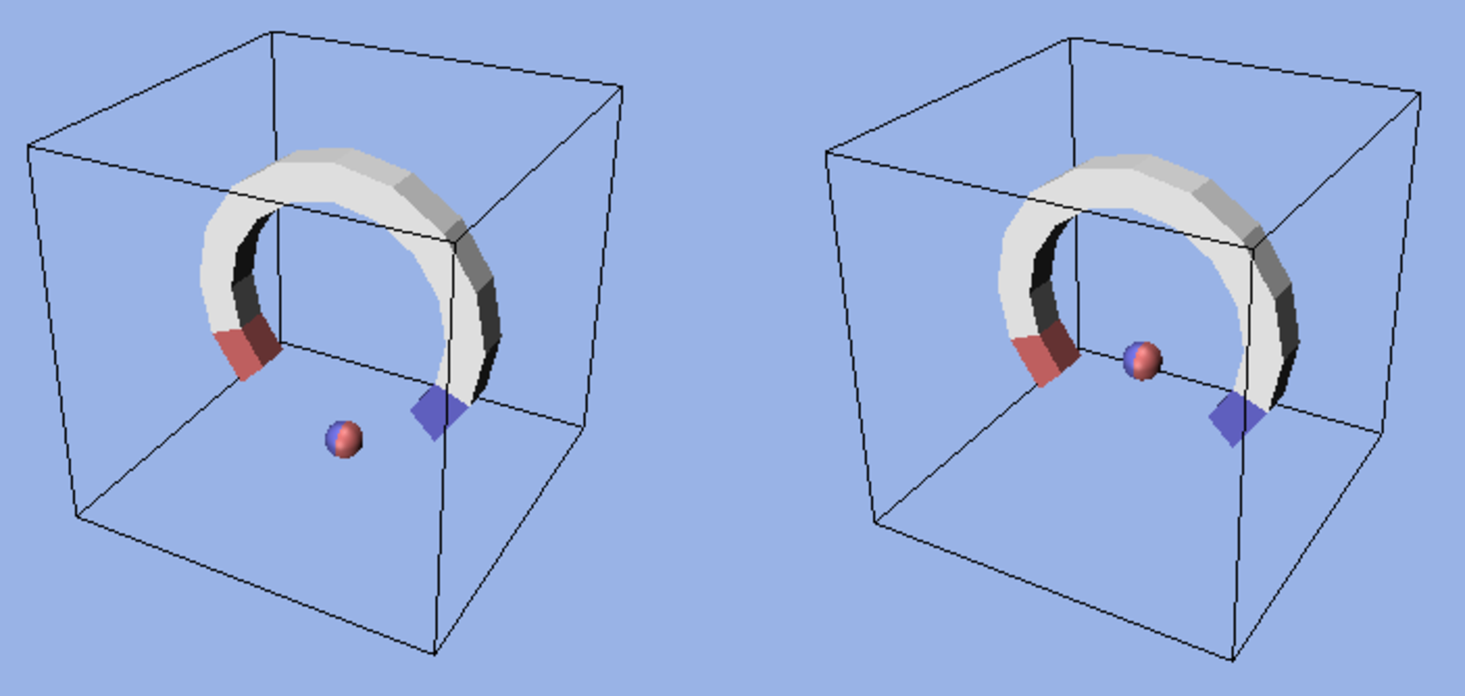
\includegraphics[width=3.0in]{images/MagnetImage3}
  \caption{A spherical magnet oscillates between the ends of a horseshoe magnet}
\end{figure}

\section{Areas for Improvement and Future Work}

As mentioned in the last section, when the magnets collide, the results are not consistent. This is because of how the penalty force method of handling collisions works. If the magnets happen to overlap only a little bit, the penalty forces will be very small, resulting in only a small bounce. If the magnets happen to overlap a lot, the penalty forces will be very large, resulting in a very violent bounce. These differences in overlap for different collisions occur because of the variations in how fast the magnets move, resulting in a difference in how far the magnets move in a single time step. This is particularly a problem when simulating magnets because the magnetic forces increase the closer the magnets are together. This can cause the magnets to accelerate to very fast speeds just before a collision.

There are a few ways this issue could be solved, or at least lessened. One way to lessen the impact of this issue is to use smaller time steps. This will result in longer simulation times, which is undesirable. Some time can be saved, however, by realizing that the small time steps are only required when the magnets collide. Checking the minimum distance between any two magnets and lowering the length of the time step only when two magnets are near each other can save some simulation time. One way to solve (and not merely reduce the impact of) this problem is to use a more physically accurate collision handling method, such as not allowing the magnets to interpenetrate at all and instead finding the exact time of the collision and handling the collision with impulses.

A related area for improvement is that contact is not handled. Currently, the magnets will continue bouncing off each other forever, instead of coming to rest in contact with each other.

When drawing the magnetic induction lines, occasionally a very long, straight line will occur due to a large magnetic induction at a point. These points occur only inside of the magnets. Thus, some work could be done to detect these extremely large magnetic induction values and not draw them, removing this incorrect visual artifact.

Although arbitrarily shaped magnets are demonstrated in the example animations, they are only implemented in the included code as objects that create a magnetic field. Collisions with these arbitrarily shaped magnets are neither detected nor handled in the included code. Additionally, the rigid body equations of motion are implemented with the assumption that the moving objects are spheres, so the arbitrarily shaped magnets are currently required to remain stationary. This is another area of future work for this project.

\section{Conclusion}

The basics of rigid body dynamics and magnetism have been presented. Though there are many improvements that can be made to the methods presented here, this report provides a useful starting point for simulating magnets.

\section*{Acknowledgements}

The author would like to thank Christopher Batty for teaching the CS888 Physically-Based Animation course this term and for the particle system starter code.

%%% Please use the ``acmsiggraph'' BibTeX style to properly format your
%%% bibliography.

\bibliographystyle{acmsiggraph}
\bibliography{template}
\end{document}
